%-------------------------------%
%  Author: Alessandro Sciarra   %
%    Date: 10 Sep 2019          %
%-------------------------------%

%~~~~~~~~~~~~~~~~~~~~~~~~~~~~~~~~~~~~~~~~~~~~%
\begin{frame}{Why do we need them?}
    \vspace{-2mm}
    \begin{itemize}
        \item In science, most of our time in the terminal is spent acting on files
        \item Mastering file handling in general can allow us to simplify the data analysis software
        \item Typical operations might be
              \begin{itemize}
                  \item Prepare data for plotting in a given format
                  \item Search patterns in a file
                  \item Extract portion of a file
                  \item Transform a file (e.g. remove trailing spaces)
                  \item \ldots
              \end{itemize}
    \end{itemize}
    \vspace{3mm}
    \begin{varblock}{}[0.95\textwidth]{GNU Core Utilities}
        \begin{tabular}{*{7}{>{\ttfamily\color{external-color}}c}}
            head    &  cat    &  sum     &  column  &  sort   &  join  &  expand   \\
            tail    &  tac    &  cksum   &  paste   &  uniq   &  comm  &  unexpand \\
                    &  cut    &  md5sum  &          &         &  tr    &  split    \\
        \end{tabular}
    \end{varblock}
    \begin{tikzpicture}[remember picture, overlay]
        \coordinate (C) at ($(current page.center)!0.5!(current page.south)$);
        \begin{scope}[every node/.style={starburst, starburst point height=6mm, fill=yellow, draw=red, ultra thick, text=red, font=\Huge\ttfamily, visible on=<2>, rotate=10}]
            \node[left  = of C, yshift=3mm] {sed};
            \node[right = of C, yshift=-1mm] {awk};
        \end{scope}
        \node[anchor=east, visible on=<2>] at ($(current page.east)+(-6mm,6mm)$) {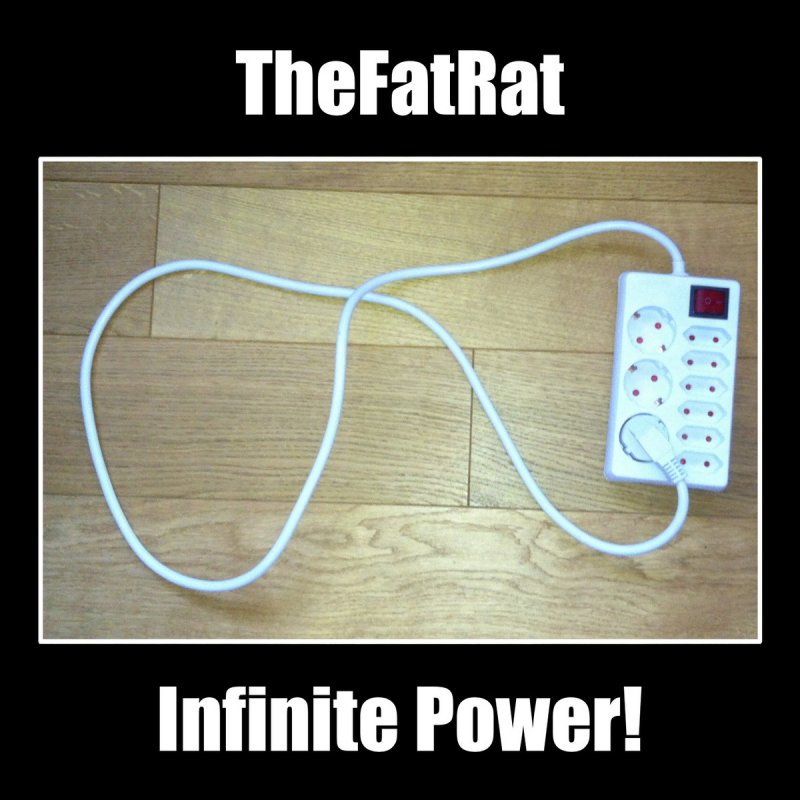
\includegraphics[width=32mm, clip, trim=1mm 3mm 1mm 48mm]{InfinitePower}};
    \end{tikzpicture}
    \PrepareURLsymbol[PB]
    \FrameRemark{A complete \URL*{https://en.wikipedia.org/wiki/List\_of\_GNU\_Core\_Utilities\_commands}{GNU coreutils list} is available on Wikipedia.}
\end{frame}
%~~~~~~~~~~~~~~~~~~~~~~~~~~~~~~~~~~~~~~~~~~~~%





